

	\chapter{Analysis and specification of requirements}

	
	\section{Introduction}
	Being the first in the development cycle of the project, this phase is the most
	important. Indeed, it is during this period that the needs of the user are identified and specified. These requirements also represent the functionalities that should be present in the application, which also makes it possible to validate the application as the development progresses.
	\section{Actors Identification}
	\textbf{MassTer Insight web Application }was mainly designed to be used by \textbf{Data Analysts }in MMM agencies, which is the case of \textbf{MASS Analytics}, \textbf{Media Agencies }that have a MMM division, and \textbf{Advertisers }who have an in-house MMM team.
	
	\clearpage
	\newpage
	
	
	\section{Requirement Analysis}

	\subsection{Functional Requirements}
     
	These functional requirements express the expectations of different users for the product to be produced.
	\\
	\\
	In this part, we present the different functionalities and services that the application must ensure.
	
	CONNECT TO SERVER
	\begin{itemize}
		\setlength{\itemindent}{+.5in}
		\item \textbf{Connect To MassTer Server : } 
	\end{itemize}
	
	LOAD PROJECT
	\begin{itemize}
		\setlength{\itemindent}{+.5in}
     	\item \textbf{Load MassTer Insight Project : } 
    \end{itemize}

	SAVE PROJECT
	\begin{itemize}
		\setlength{\itemindent}{+.5in}
		\item \textbf{Save MassTer Insight Project : } 
	\end{itemize}

	SAVE AS PROJECT
	\begin{itemize}
		\setlength{\itemindent}{+.5in}
		\item \textbf{Save as MassTer Insight Project : } 
	\end{itemize}


	
 
 	MANAGE REPORT
 		\begin{itemize}
 			\setlength{\itemindent}{+.5in}
 			\item \textbf{Load a Report : } 
 			\item \textbf{Save a Report : }
 			\item \textbf{Remove a Report : }
 	\end{itemize}
 
  	UPDATE SETTINGS
    \begin{itemize}
    	\setlength{\itemindent}{+.5in}
    	\item \textbf{Update Settings Report : }
   \end{itemize}

  	RUN
   \begin{itemize}
   	   \setlength{\itemindent}{+.5in}
 	   \item \textbf{Run new scenario : }
   \end{itemize}

    \clearpage
    \newpage

	\subsection{Non-Functional Requirements}
	\begin{itemize}
		\item \textbf{Ergonomics : }The application offers a user-friendly and easy-to-use interface without refer to particular knowledge.
		\item \textbf{Security : ????}
		\item \textbf{Scalability : ????}
		\item \textbf{Modularity : }a code that is easy to maintain and simple to understand in order to ensure the scalability of application. 
	\end{itemize}
	\clearpage
	\newpage
	
	\section{Use Case Diagrams}
	\subsection{Global Use Case Diagram}
	\begin{figure}[h]
		\centering
		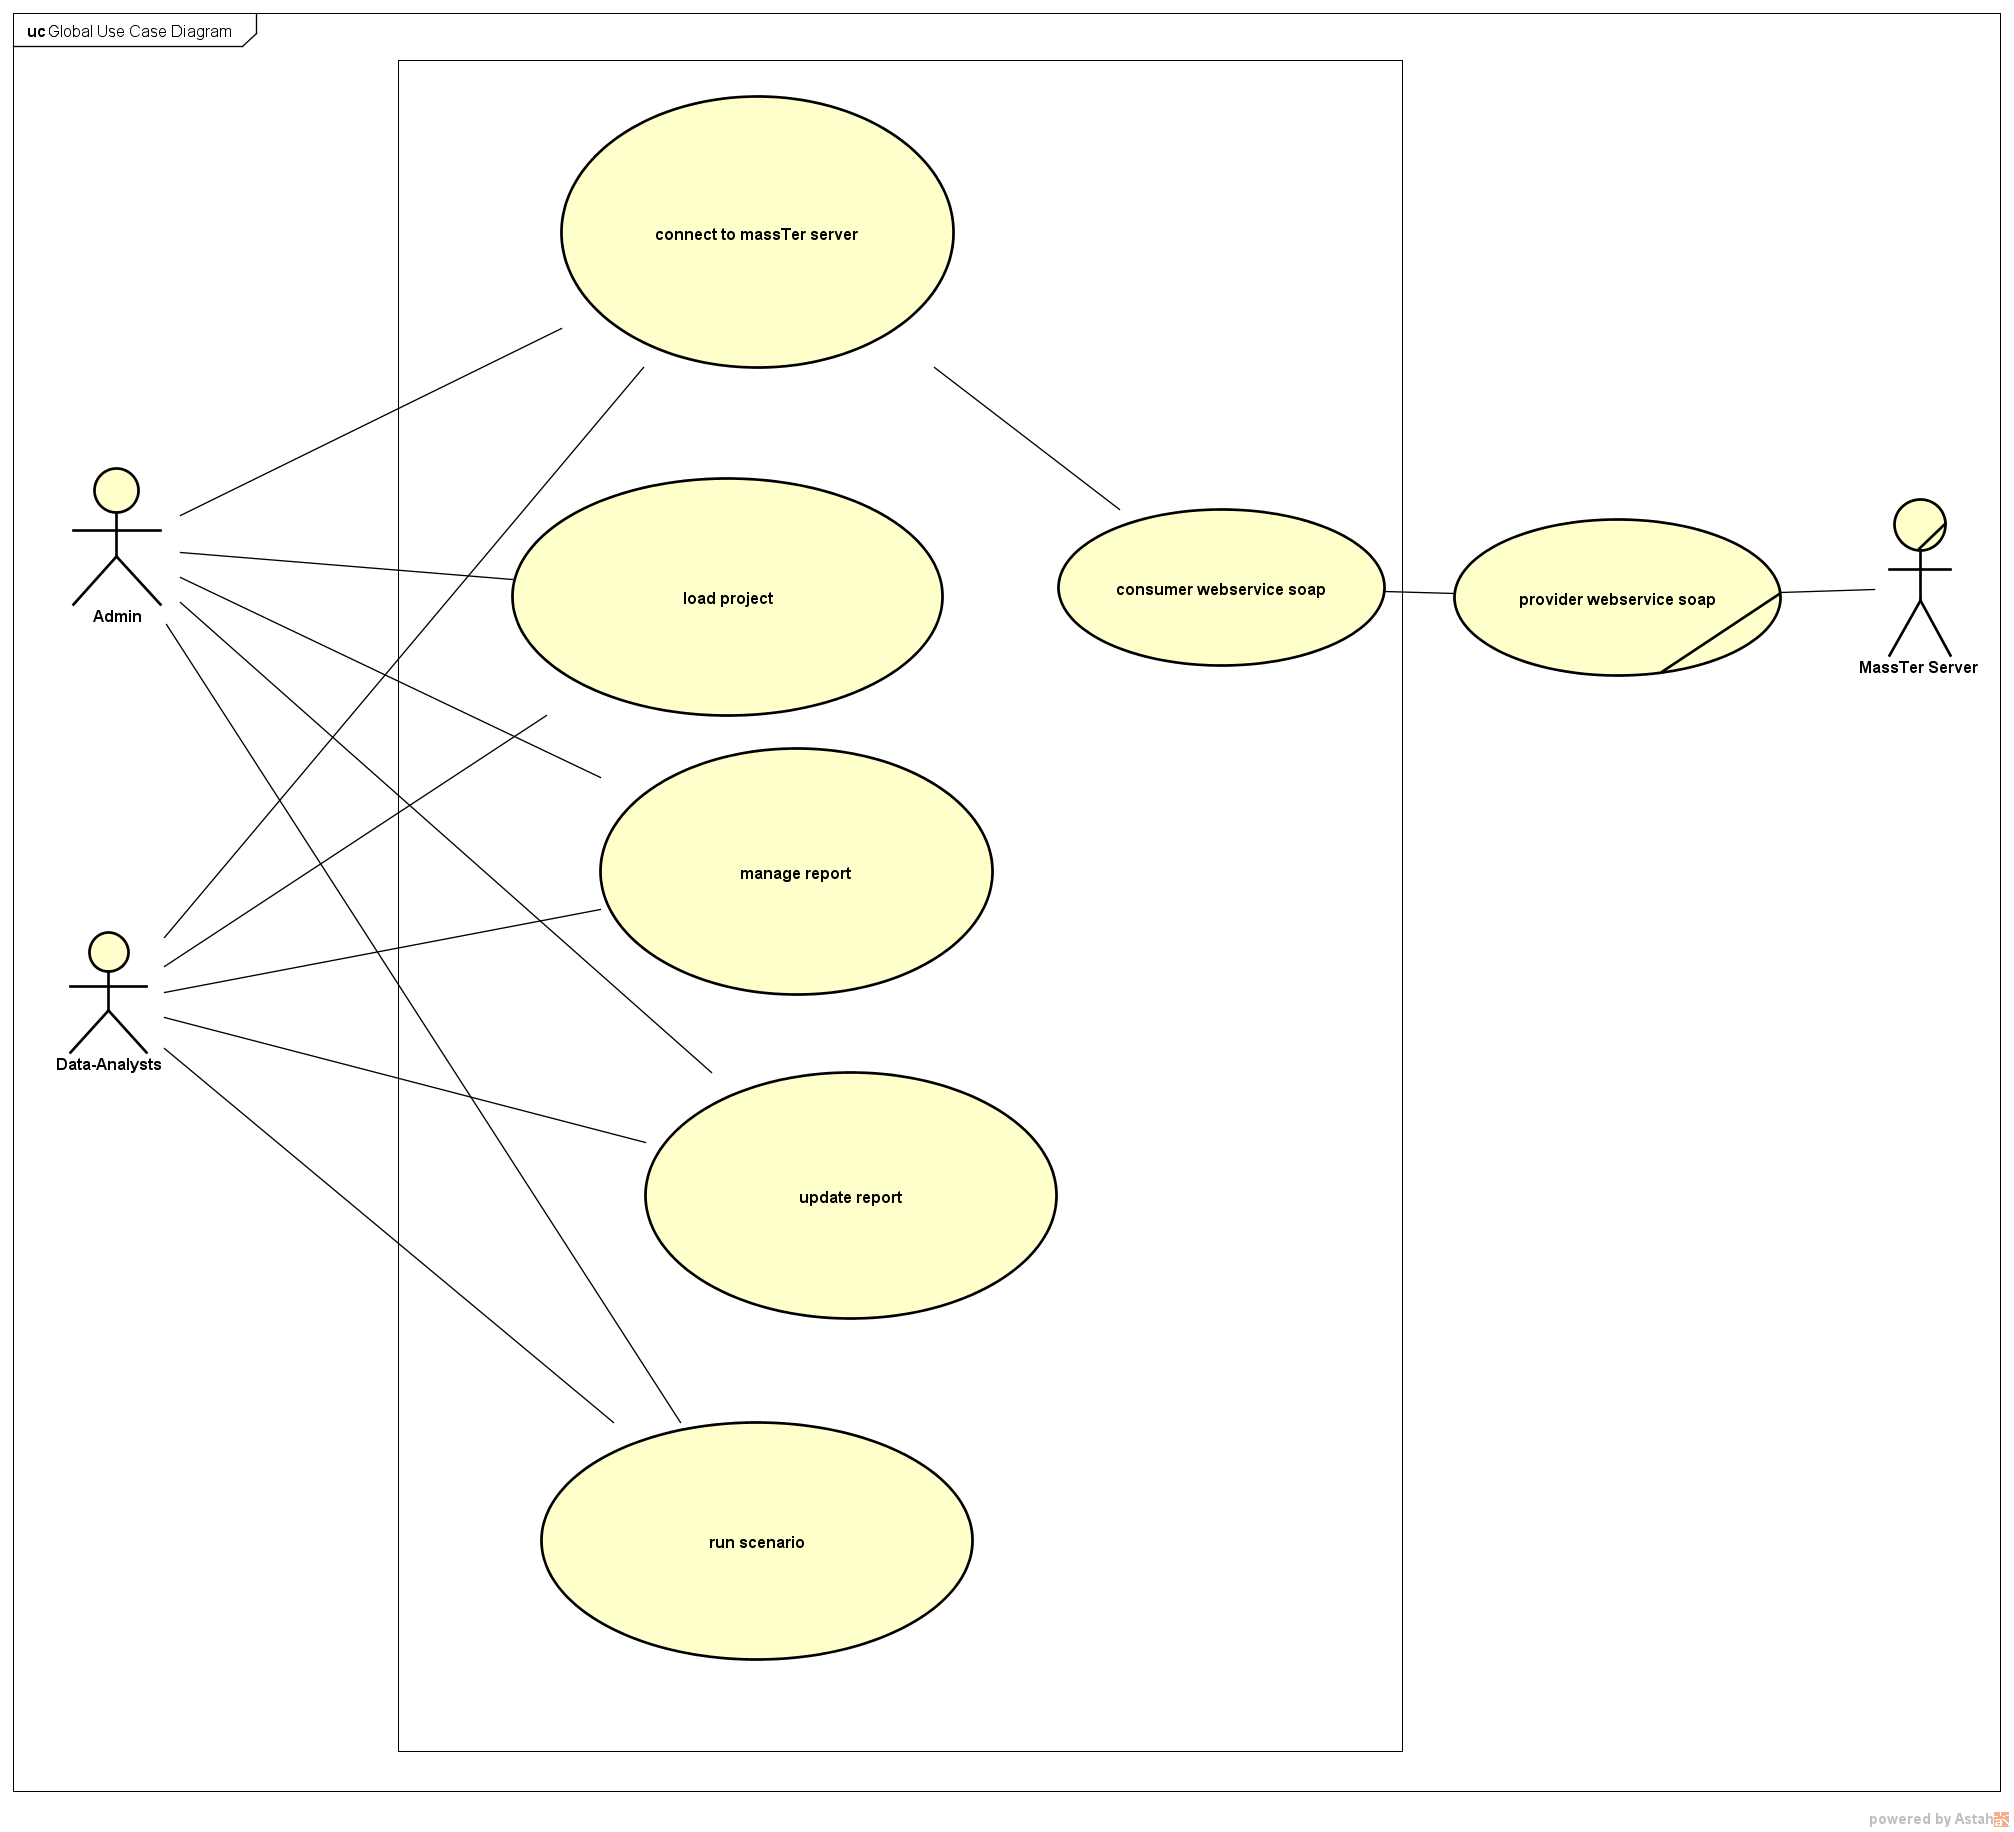
\includegraphics[width=16.5cm,height=16cm]{GlobalUseCaseDiagram.png}
		\caption{Global Use Case Diagram}
		
	\end{figure}

\clearpage
\newpage

	\subsection{Detailed Use Case Diagrams}
	 \subsubsection{Connect to MassTer Server Use Case}
	 \begin{figure}[h]
	 	\centering
	 	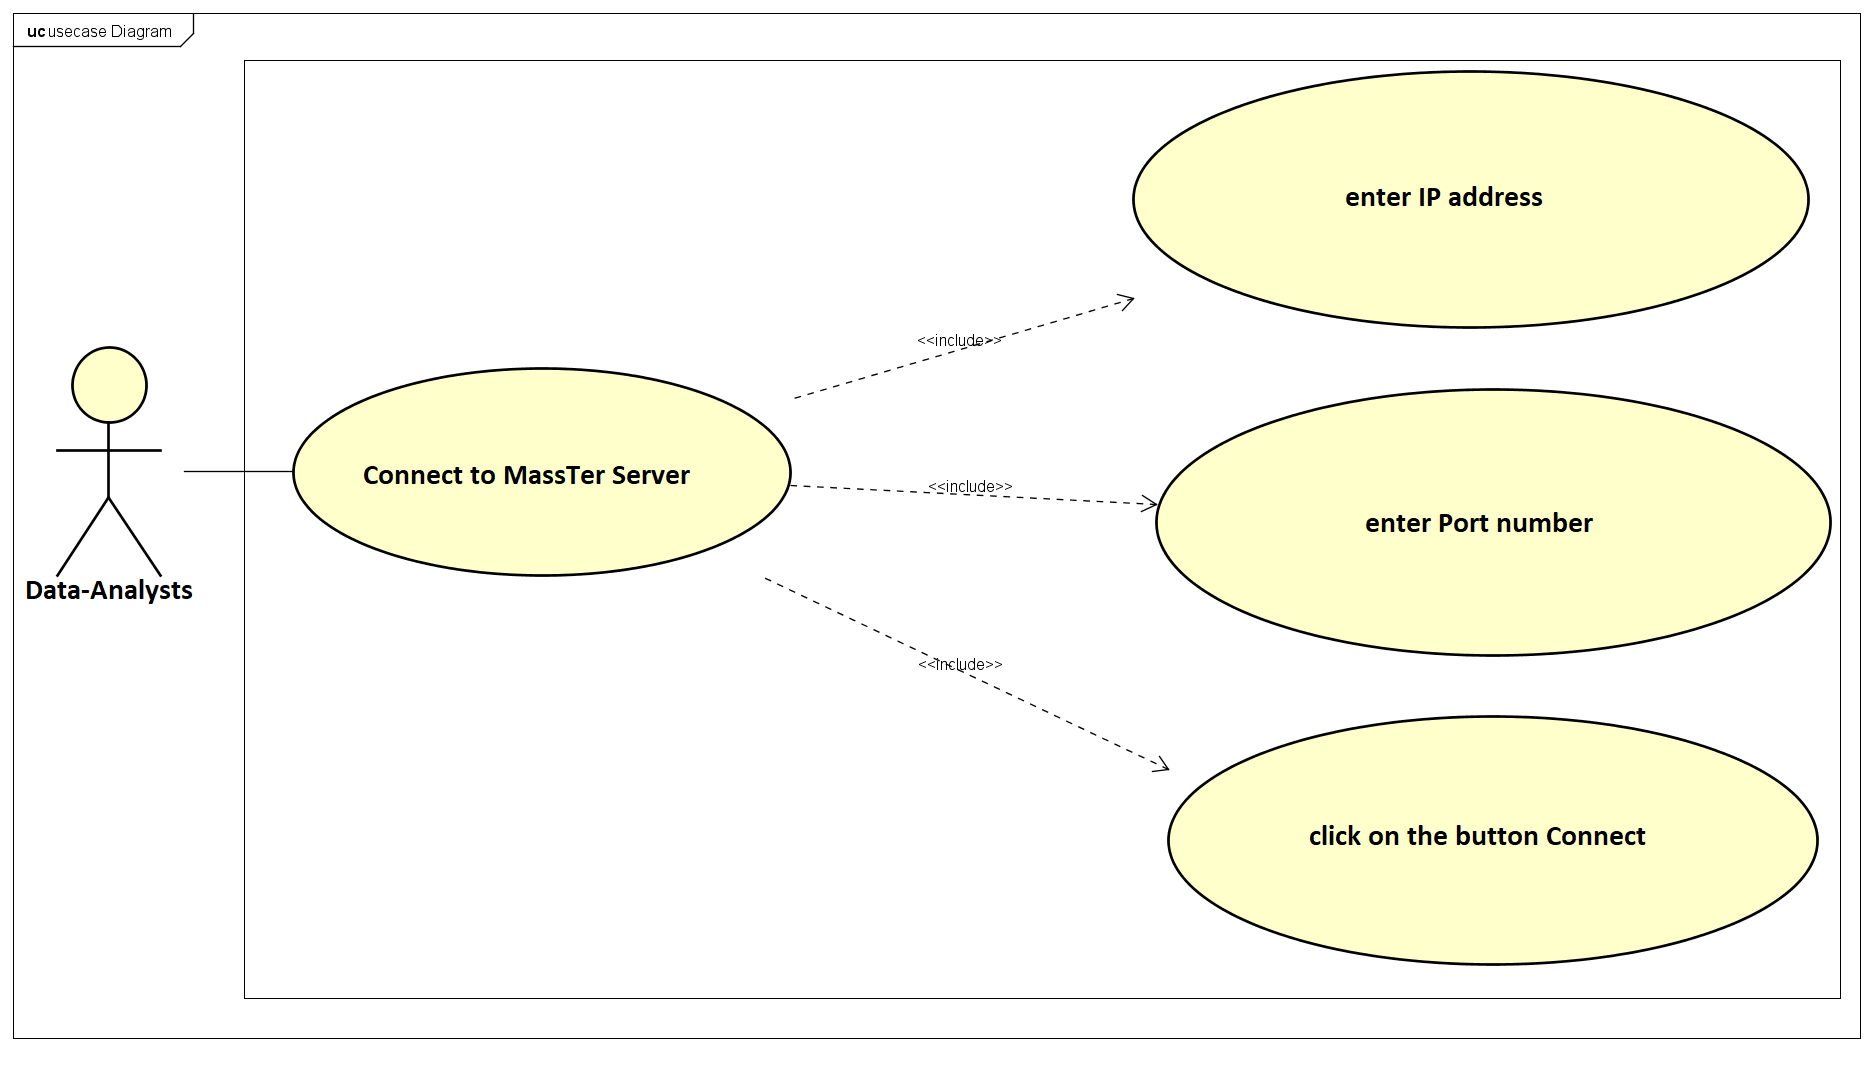
\includegraphics[width=16.5cm,height=10cm]{connectToMassTerServer.png}
	 	\caption{Connect to MassTer Server Use Case Diagram}
	 	
	 \end{figure}

  \newpage
 
 \begin{table}
 	\caption{Description of the scenario \textbf{Connect to MassTer Server Use Case}.}
 	\label{DSTabCTMS}
 	\centering
 	
 	\begin{tabular}{|c|p{10cm}|}
 		\hline 	
 		\textbf{Pre-Conditions } & MassTer Server is running  \\ 
 		\hline                     
 		\textbf{Nominal Scenario } & \begin{enumerate}
 			\item The user click on the item MassTer Server in Main Menu.
 			\item The Application display a drop down. 
 			\item The user type MassTer Server IP address.
 			\item The user type MassTer Server port number.
 			\item The  user click on button connect. 
 		\end{enumerate} \\ 
 		\hline 
 		\textbf{Post-Conditions} & Connect to MassTer Server is successfully. \\
 		\hline 
 	\end{tabular}
 \end{table}
 \clearpage
 \newpage
	 \subsubsection{Load Project Use Case}
	 	\begin{figure}[h]
	\centering
	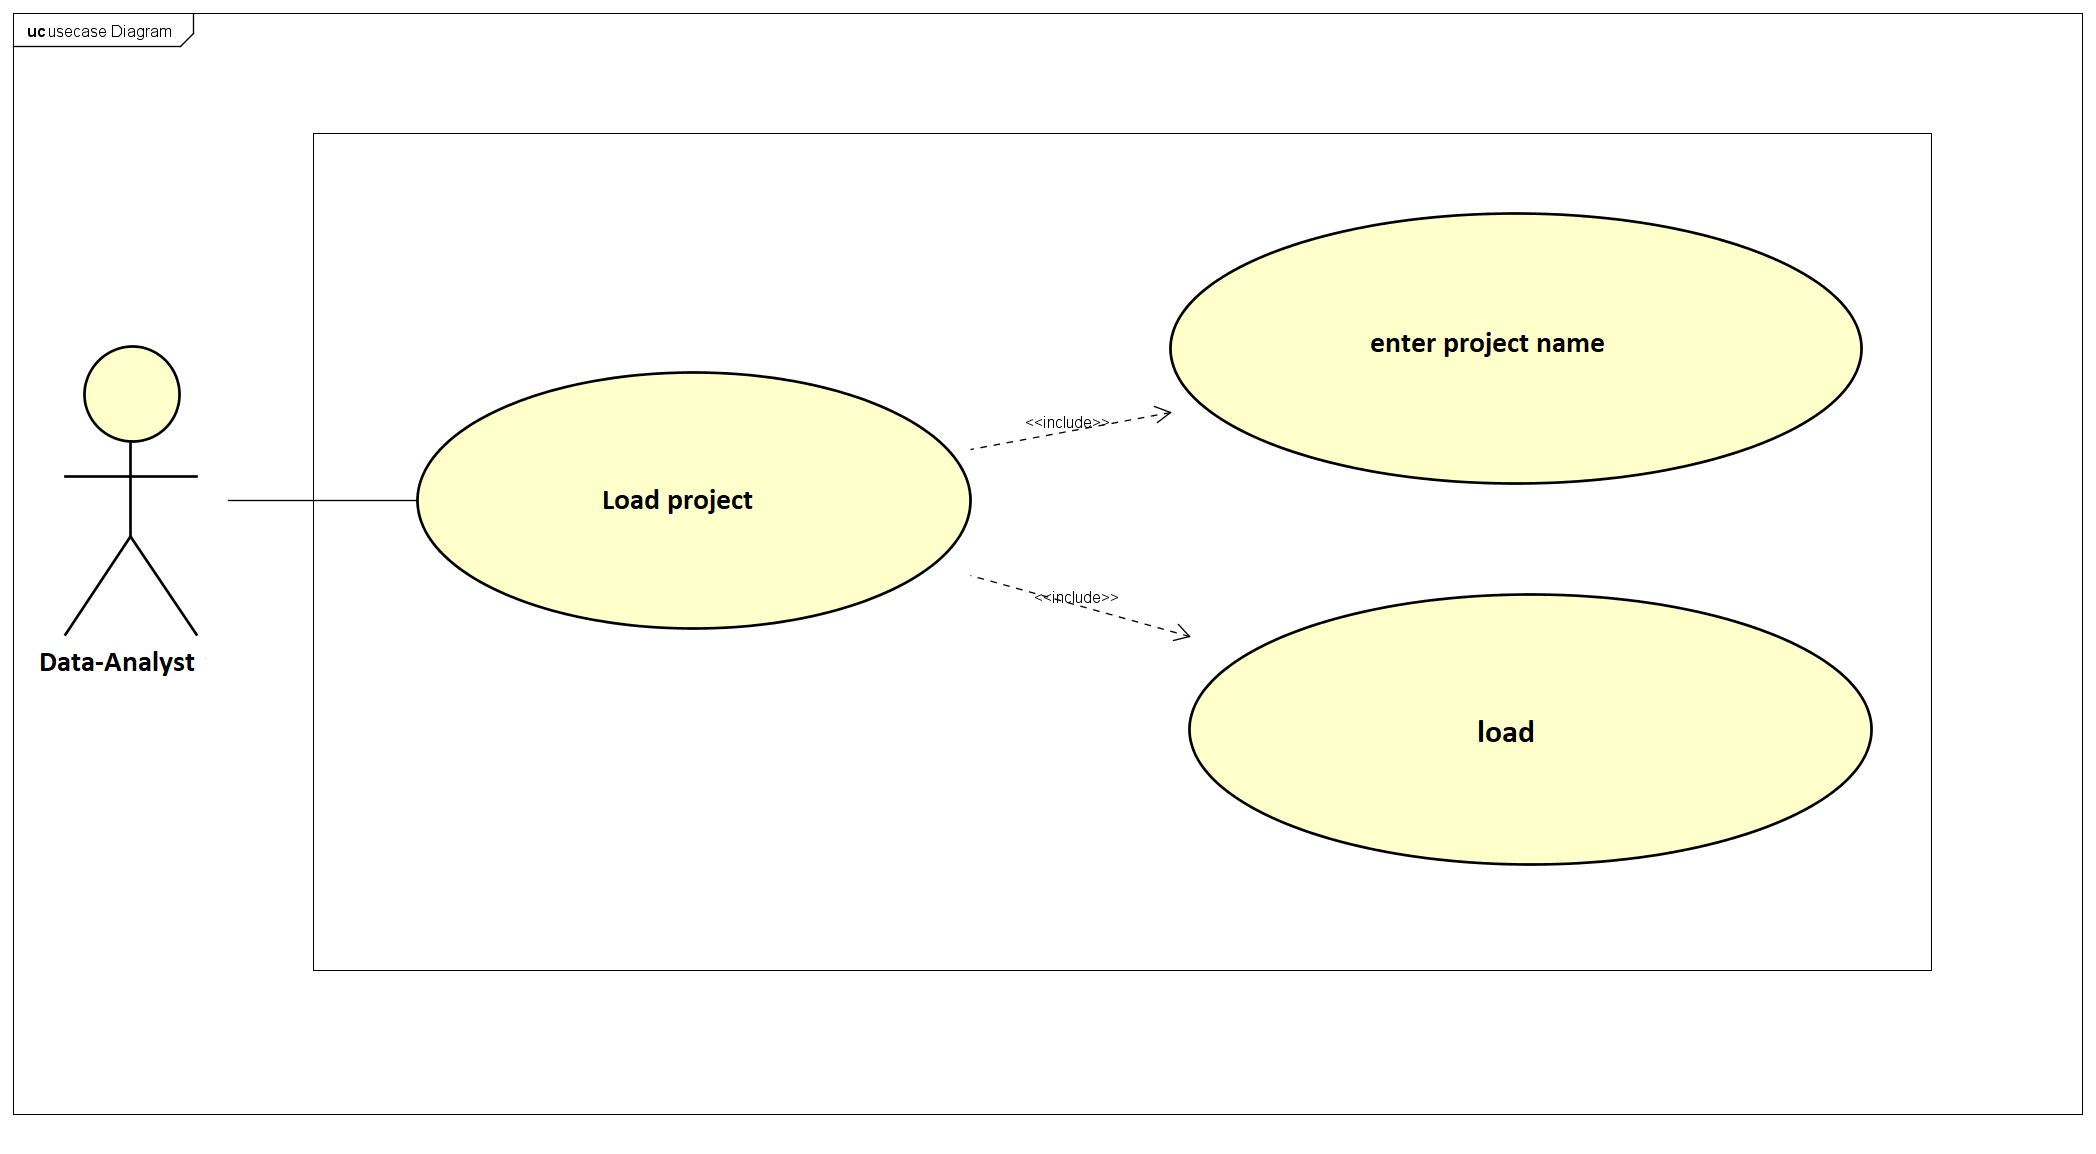
\includegraphics[width=16.5cm,height=9cm]{loadProject.png}
	\caption{Load Project Use Case Diagram}
	
	\end{figure}
 
  \begin{table}
  	\caption{Description of the scenario \textbf{Load Project Use Case}.}
  	\label{DSTabLP}
 	\centering
 	\begin{tabular}{|c|p{10cm}|}
 		\hline 	
 		\textbf{Pre-conditions } & MassTer Server is running \\ 
 		\hline                     
 		\textbf{Nominal Scenario } & \begin{enumerate}
 			\item The user click on the item Load project in Main Menu.
 			\item The user type MassTer Insight project name.
 			\item The user click on the button load. 
 		\end{enumerate} \\ 
 		\hline 
 		\textbf{Post-conditions} & The Application display optimization page. \\
 		\hline 
 	\end{tabular}
 \end{table}

  \begin{table}
	\caption{Description of the scenario \textbf{Save Project Use Case}.}
	\label{DSTabSP}
	\centering
	\begin{tabular}{|c|p{10cm}|}
		\hline 	
		\textbf{Pre-conditions } & \begin{enumerate}
			\item MassTer Server is running.
			\item Load Project is done successfully.
		\end{enumerate}  \\ 
		\hline                     
		\textbf{Nominal Scenario } & \begin{enumerate}
			\item The user click on the item save project in Main Menu.
			\item The user select save item in the drop down.
		\end{enumerate} \\ 
		\hline 
		\textbf{Post-conditions} & the project is saved successfully. \\
		\hline 
	\end{tabular}
\end{table}
   \begin{table}
 \caption{Description of the scenario \textbf{Save As Project Use Case}.}
 	\label{DSTabSAP}
 	\centering
 	\begin{tabular}{|c|p{10cm}|}
 		\hline 	
 		\textbf{Pre-conditions } & \begin{enumerate}
 			\item MassTer Server is running.
 			\item Load project is done successfully.
 		\end{enumerate} \\ 
 		\hline                     
 		\textbf{Nominal Scenario } & \begin{enumerate}
 			\item The user click on the item save as in Main Menu.
 			\item The user select save as item in the drop down.
 		\end{enumerate} \\ 
 		\hline 
 		\textbf{Post-conditions} & The project is saved with a new name successfully. \\
 		\hline 
 	\end{tabular}
 \end{table}
\clearpage
\newpage

 
 \subsubsection{Manage Report Use Case}
	 	\begin{figure}[h]
	\centering
	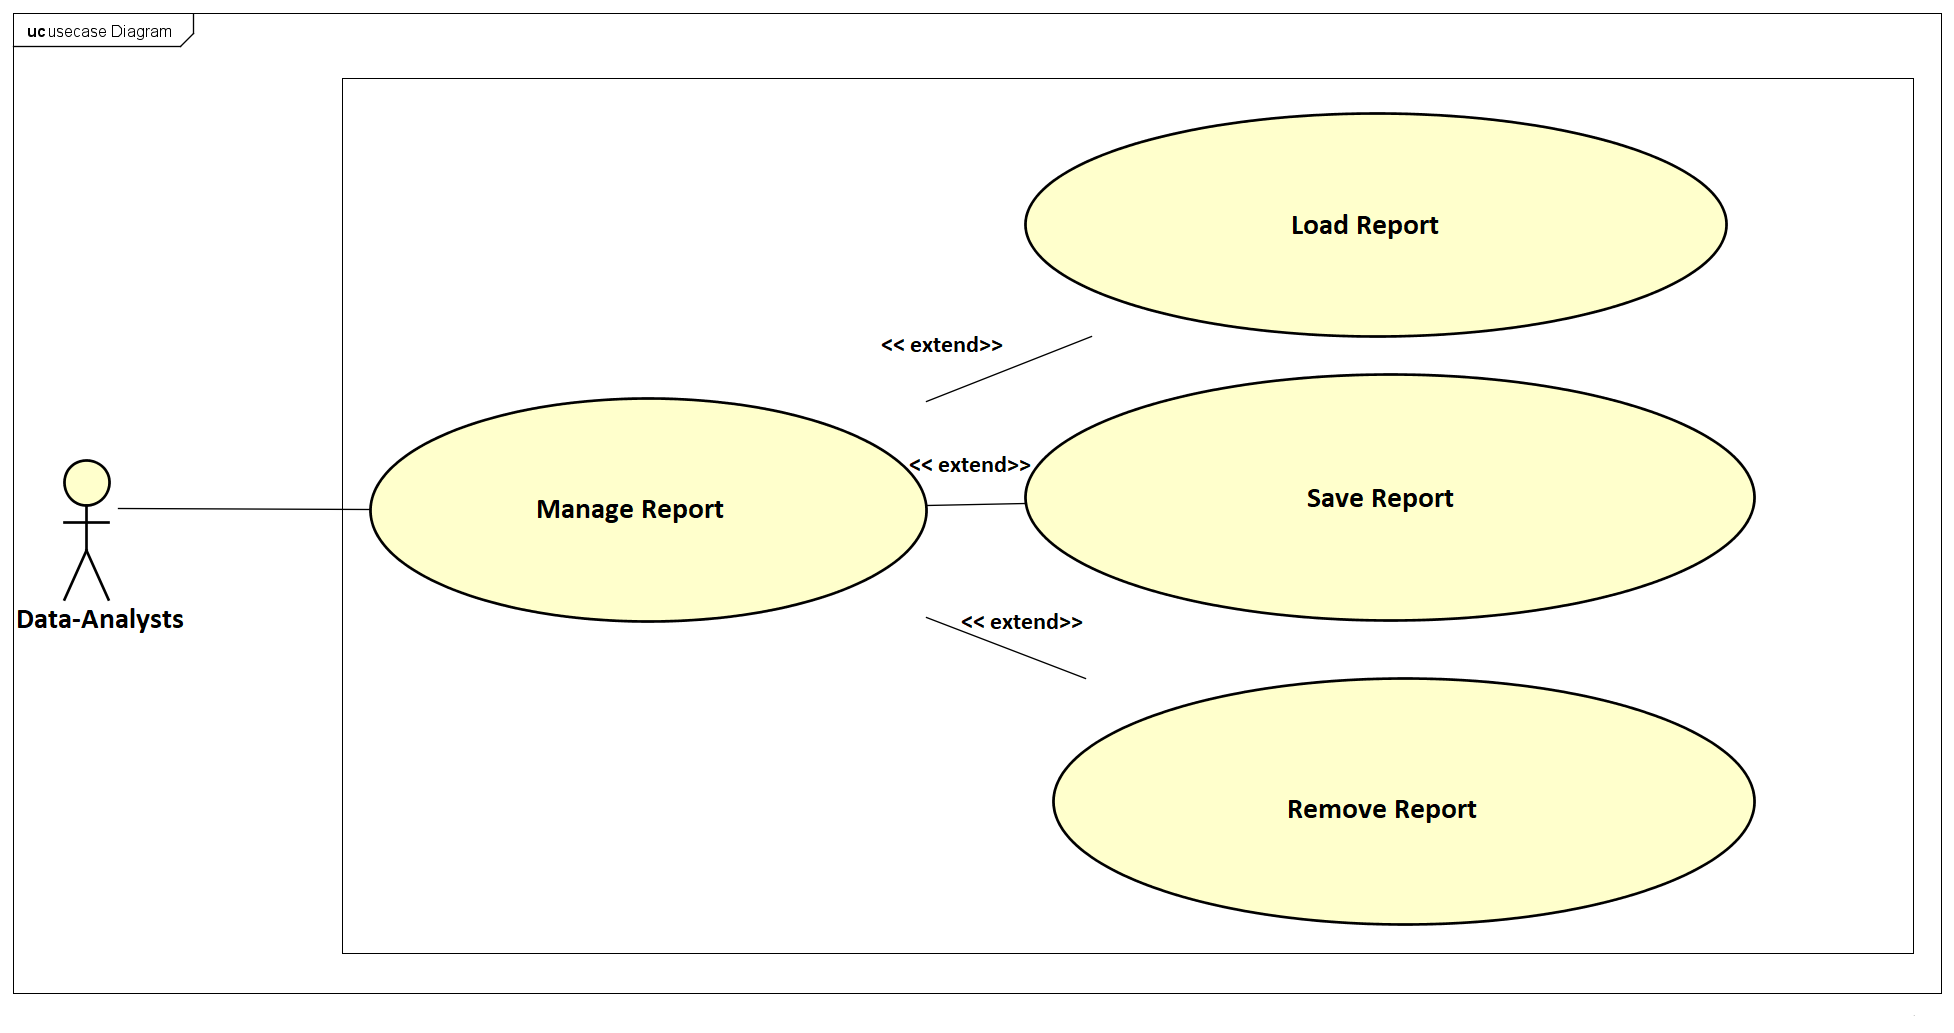
\includegraphics[width=16.5cm,height=9cm]{manageReport.png}
	\caption{Load Project Use Case Diagram}
	
\end{figure}

 \begin{table}
 	\caption{Description of the scenario \textbf{load report Use Case}.}
 	\label{DSTabLR}
 	\centering
 	\begin{tabular}{|c|p{10cm}|}
 		\hline 	
 		\textbf{Pre-Conditions } & MassTer Server is running \\ 
 		\hline                     
 		\textbf{Nominal Scenario } &  \begin{enumerate}
 			\item The user select a report from the drop down.
 			\item The user click on the button load.
 		\end{enumerate} \\ 
 		\hline 
 		\textbf{Post-Conditions} & The application display a new optimisation report related to the selected report \\
 		\hline 
 	\end{tabular}
 \end{table}
 
 \begin{table}
 	\caption{Description of the scenario \textbf{Save Report Use Case} .}
 	\label{DSTabSR}
 	\centering
 	\begin{tabular}{|c|p{10cm}|}
 		\hline 	
 	\textbf{Pre-Conditions } & MassTer Server is running\\ 
 	\hline                     
 	\textbf{Nominal Scenario } & \begin{enumerate}
 		\item The user click on the button save.
 			\item The user type a name for the new report in the pop up.
 		\item The user click on the button save in the pop up.
 	\end{enumerate} \\ 
 	\hline 
 	\textbf{Post-Conditions} & \begin{itemize}
 			\item The drop down refresh the list of reports.
 	    	\item Add the new report to the list of reports.
 	\end{itemize}\\
 	\hline  
 	\end{tabular}
 \end{table}
 
 \begin{table}
 	\caption{Description of the scenario \textbf{Remove Report Use Case}.}
 	\label{DSTabRR}
 	\centering
 	\begin{tabular}{|c|p{10cm}|}
 		\hline 	
 		\textbf{Pre-Conditions } & MassTer Server is running\\ 
 		\hline                     
 		\textbf{Nominal Scenario } & \begin{enumerate}
 			\item The user select a report from the drop down.
 			\item The user click on the button remove.
 		\end{enumerate} \\ 
 		\hline 
 		\textbf{Post-Conditions} & \begin{itemize}
 			\item The selected report was deleted.
 			\item The drop down refresh the list of reports.
 			\item Removes the deleted report from the list.
 		\end{itemize}\\
 		\hline 
 	\end{tabular}
 \end{table}
  
    \begin{table}
    	\caption{Description of the scenario \textbf{update settings Use Case}.}
    	\label{DSTabUS}
  	\centering
  	\begin{tabular}{|c|p{10cm}|}
  	
  		\hline 	
  		\textbf{Pre-conditions } &The loaded MassTer Insight project contains at least one report saved \\ 
  		\hline                     
  		\textbf{Nominal Scenario } & \begin{enumerate}
  			\item The user select new channels .
  			\item The user click on the button update.  
  		\end{enumerate} \\ 
  		\hline 
  		\textbf{Post-conditions} & The Application display a pop up notification to inform the user that the update was done successfully. \\
  		\hline 
  	\end{tabular}
  \end{table}

	 	\begin{figure}[h]
	 	\centering
	 	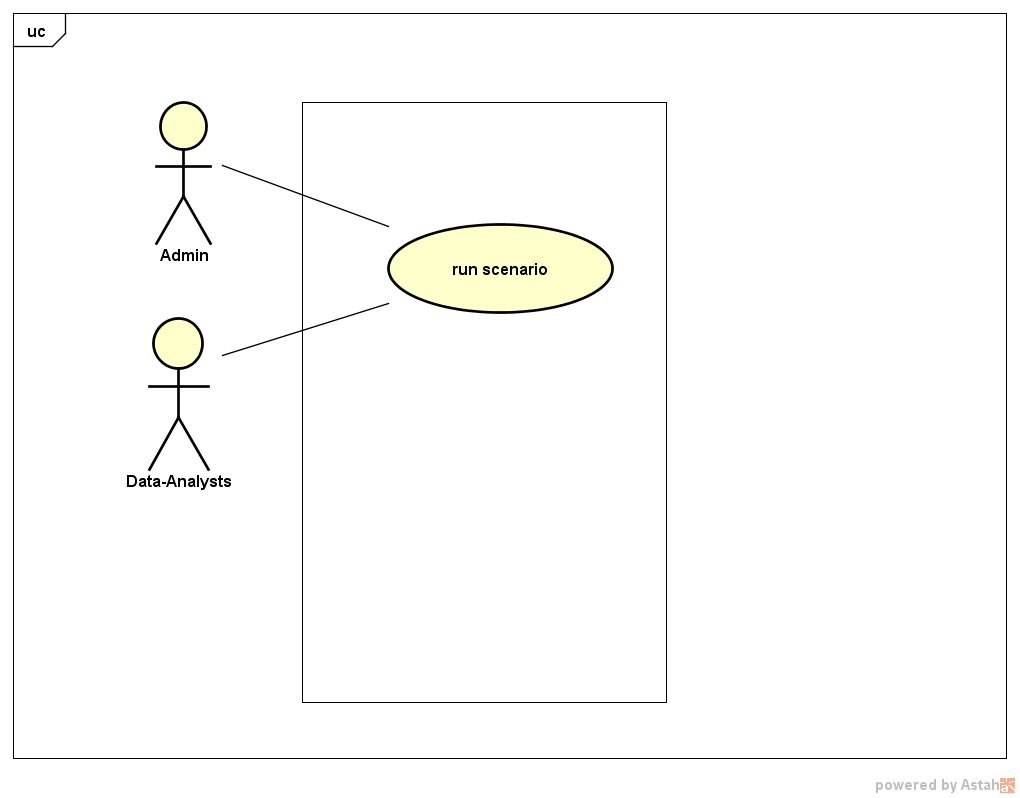
\includegraphics[width=16.5cm,height=11cm]{runScenario.png}
	 	\caption{run scenario Use Case Diagram}
	 	
	 \end{figure}
	
	\begin{table}
			\caption{Description of the scenario \textbf{Run Scenario Use Case}.}
		\label{DSTabRS}
		\centering
		\begin{tabular}{|c|p{10cm}|}
			\hline 	
			\textbf{Pre-conditions } & The update was done with success \\ 
			\hline                     
			\textbf{Nominal Scenario } & \begin{enumerate}
				\item The user check max Budget or min Target.
				\item The user type new value for radio checked.
				\item The user type the budget Range.
				\item The user type the resolution.
				\item the user modifier the constraints table.
				\item The user click on the button run. 
			\end{enumerate} \\ 
			\hline 
			\textbf{Post-conditions} & The Application display a new optimisation report with new Optimisation Results. \\
			\hline 
		\end{tabular}
	\end{table}
	\clearpage
	\newpage
	
	\section{Conclusion}
	This chapter has allowed us to identify the actors that may interact with the developed system, to define the functional and non-functional requirements of the project and modeling the use case diagrams.
	\\
	In what follows, we present the general and detailed conception phase of the System.  
	
